\documentclass[11pt]{jarticle}

\usepackage{amsmath}
\usepackage{graphics}
\usepackage{hyperref}

\setlength{\oddsidemargin}{-0.7cm}
\setlength{\topmargin}{-1.5cm}
\setlength{\textwidth}{16.5cm}
\setlength{\textheight}{26cm}
\pagestyle{empty}

\begin{document}

\noindent
{\bf\large 「計算機実験II」実習課題(EX2) 2017-11-10}
\\[-0.5em]

\noindent
\begin{itemize}
\item 講義のページ: \verb+http://exa.phys.s.u-tokyo.ac.jp/ja/lectures/2017W-computer2+

\item サンプルプログラム: \\ {\small \verb+https://github.com/todo-group/computer-experiments/releases/tag/2017-2-L1+}からexample-2-L2.zipをダウンロードして展開する

\item 準備練習
  
  \begin{enumerate}
  \item {\tt example-2-L2/random.c}は、Mersenne-Twister 乱数発生器 (mersenne twister.h) により、(0, 1) の範囲で一様分布する実数乱数を生成するプログラムである。種(seed)を変えて何度か乱数を生成し、その時系列を比較してみよ
  \end{enumerate}

\item 基本課題
  \begin{enumerate}
  \item
    \begin{itemize}
    \item サンプルプログラム{\tt example-2-L2/histogram.c}は、$(0,1)$の一様乱数を生成し、そのヒストグラムを出力するプログラムである。コンパイル・実行し、下のようなグラフを作成してみよ
      \begin{center}
        \resizebox{.5\textwidth}{!}{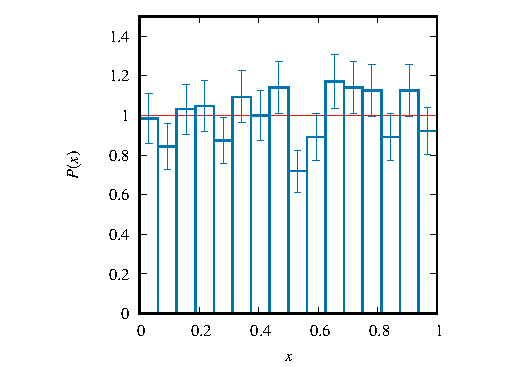
\includegraphics{histogram.eps}}
      \end{center}
    \item $X$と$Y$を$(0,1)$で一様分布するそれぞれ独立な(実数)確率変数とする。このとき$X^2$, $-log X$, $XY$のそれぞれの確率密度関数と期待値を(解析的に)求めよ。また、実際に乱数を生成させてヒストグラムと期待値を計算し、解析的な結果と比較せよ
    \end{itemize}
    \item 
    \begin{itemize}
    \item 棄却法により、確率密度関数
      \begin{equation}
        P(x) = \begin{cases} 4x & 0 < x < 1/2 \\
          4(1-x) & 1/2 < x < 1 \\
          0 & \text{otherwise}
        \end{cases}
        \label{eqn:triangle}
      \end{equation}
      にしたがう一様乱数を生成せよ。ヒストグラムを作り、結果を確認せよ
    \item 確率密度関数(\ref{eqn:triangle})にしたがう$m=10$個の独立な確率変数の平均$Y=(1/m) \sum_{i=1}^m X_i$のヒストグラムを調べよ。$m$を増やしていくと分布はどのような形に近づくだろうか? 理論の予想と比較してみよ
    \end{itemize}
  \end{enumerate}  
\item 応用課題
  \begin{enumerate}
  \item 正規分布にしたがう乱数の生成方法について調べよ。また、平均値$\mu_i$と分散共分散行列$\Sigma_{ij}$をもつ多次元正規分布にしたがう乱数の生成方法を考えよ
  \end{enumerate}

\item レポート課題

  基本課題?についてレポートを作成し提出せよ(基本課題?はオプション)。実習1 (EX1)のレポート課題とあわせて、一つのレポートとして提出すること。提出締め切りは12月1日とする。提出方法...
  
\end{itemize}

\end{document}
